\chapter{Marcos WORKS!}

\subsection{LED}
For illuminating the scene, several different alternative were discussed and ultimately IR LEDs were chosen \fxnote{Refer to the chapter in which this is discussed} because of their good illumination outside of the visible spectrum. For the project two different LEDs were tested, both emitting at roughly 880nm \fxnote{need source datasheet at chosen led: http://www.komponenten.es.aau.dk/fileadmin/komponenten/Data_Sheet/Opto/SFH484_485.pdf the other one we tested at http://www.komponenten.es.aau.dk/fileadmin/komponenten/Data_Sheet/Opto/SFH487P.pdf}. A 5mm with a cone of light of 16 degrees\fxnote{source is datasheet} and a 3mm with a cone of light of 130 degrees\fxnote{source is datasheet}. \fxnote{get pictures for both of these}

During initial testing the focussed beam from the 5mm LED looked as though it might be too focussed, making it  difficult to create a bright line of unbroken illumination. For that reason a series of experiments were conducted: A setup that tested the light that the two LEDs offered \fxnote{refer to image} were constructed and it was apparant that the broader LEDs did not focus the light enough, and thus did not create a high enough illumination. Therefore the choice was made to go with the 5mm, 16 degree LEDs.

Initially a broader strip of light was thought to be desirable, therefore a test was conducted where the LEDs had their lens sanded down in order to make the light less focuessed. Figure \fxnote{insert correct picture} shows an image where the LEDs in progression from left to right get more and more sanded down. As the figure illustrates the intensity of the light decreases as the LED-lens is sanded down. After conducting these tests,  it became clear that an unaltered LED performed better than the modified ones, providing a more intense illumination.

For ease of construction the LEDs were arranged into arrays of 8 LEDs connected in series, which in turn are connected in parrallel. The LEDs have a forward voltage of 1.5V, which means that the power supply has to be able to supply at least 12V to them. Initially a small AC-DC power supply capable of supplying 600mA was used for testing purposes. However the total draw of the LED array is 0,5A and for the project a total of 4 arrays were planned. The current far exceeded what could be supplied by the small AC-DC suplly. Luckily the group managed to salvage a 300 watt computer power supply capable of supplying 12 volts at 8 amperes. After getting the power supply to work without being in a computer, terminals were soldered to LED-strips and the power supply allowing the LED-strips to plug into the power supply.

\subsection{Techincal description of median and mean filters}

\subsubsection{Mean filter}
One method of filtering is the mean filter. As the name implies a mean filter takes a input image, calculates the mean value of a given pixel and uses this as the output, a mean filter is a type of neighborhood processing. In practical application this means that the average of the input pixel and the surrounding pixels decides the value of the output pixel, see figure \ref{fig:neigh_pros}.

\begin{figure}[htbp] 
\centering 
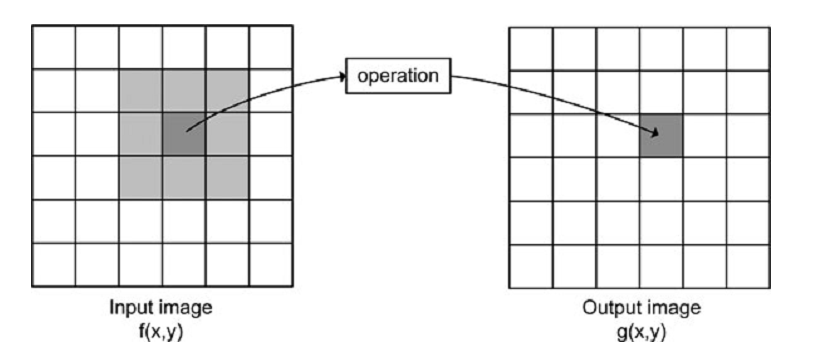
\includegraphics[width=0.5\textwidth]{Pictures/Theory/neighborhood_processing.png} 
\caption{Practical neighborhood processing. All the surrounding pixels contribute to the average value of the output.} 
\label{fig:neigh_pros} 
\end{figure}

The calculations that lie behind the average are simple:

$
\frac{\text{Sum of input- and neighboring pixels}}{\text{number of pixels}}
$

\subsubsection{Median filter}
Another method of filtering is the median filter. The median once again relies on the neighboring pixels. By indexing the input pixel along with its neighbors in a ordered list and choosing the middle value, i.e. the \textit{mean}, the output pixel is determined. In practical applications the algorithm required for a median filter can be broken down in to two steps: Creating a ordered list of the pixels and finding the mean value.

Taking out input pixels, $n_1$ through $n_9$ we first create a ordered list:
$
\text{Ordered list:}\sqsubset n_1,n_2,n_3,n_4,n_5,n_6,n_7,n_8,n_9 \sqsupset
$
Then we find the median:
$
\text{Mean}\sqsubset n_1,n_2,n_3,n_4,\textbf{n_5},n_6,n_7,n_8,n_9 \sqsupset
$